\documentclass{article}

\usepackage{inputenc}
\usepackage{csquotes}
\usepackage[a4paper, total={6in, 10in}]{geometry}
\usepackage{hyperref}
\usepackage{amsmath,amssymb}
\usepackage{graphicx}
\usepackage{indentfirst}
\usepackage{caption}
\usepackage{subcaption}
\usepackage{tikz}
\usetikzlibrary{decorations.pathreplacing,positioning, arrows.meta}

\usepackage[backend = biber,
		   style = authoryear,
		   maxnames = 5,
		   maxcitenames = 2,
		   doi = false,
		   eprint = false]{biblatex}

\addbibresource{biblio.bib}

\title{The effect of minimum wage on rents and amenities}
\author{\textit{Gabriele Borg} \and
    \textit{Diego Gentile Passaro} \\	\small Brown University
    \and \textit{Santiago Hermo}}

\begin{document}

	\maketitle
	
\section{Introduction}\label{sec:intro}

The growing disparity in income and opportunities across the US is becoming one of the most pressing issues of modern society. The complexity of both causes and consequences has been faced with a wide spectrum of both \textit{place-} and \textit{person-based} policy tools, but what are the the first-order impacts of many of them is still an open question. Focusing on the former, in recent years many US jurisdictions have adopted minimum wage laws (hereafter MW) setting workers' hourly pay above the federal minimum of \$7.25.\footnote{As of January 2020, there were 29 states with a minimum wage higher than the federal one, 52 counties with a MW above the state's, and 15 cities with a MW above the county's.} Despite a prominent debate around recent MW policies both at local and national level, starting from the seminal work of \textcite{card2000minimum}, most research effort has been directed towards understanding the effects of MW on employment \parencite[e.g,][]{dube2010minimum, neumark2006minimum, cengiz2019effect}. This is not surprising, as employment effects are of first order importance to understand the welfare implications of MW changes. However, as non-federal MW changes are \textit{place-based} by definition, it is also natural to expect these changes affecting households' welfare through markets other than the labor one. A very likely candidate to experience such effects is the housing market: How do local rents and prices react to MW changes? Surprisingly, there is very little research estimating the effects of MW on rents and house values, and virtually no research estimating the effects on local amenities.\footnote{To our knowledge the only papers aiming at answering this question are \textcite{yamagishi2019minimum} and \textcite{tidemann2018mw}. Surprisingly, they both found opposing results despite using the same year-county data. \textcite{yamagishi2019minimum} find a small positive effect, while \textcite{tidemann2018mw} finds a small negative effect. \textcite{yamagishi2019minimum} attributes this difference to different model specifications, and argues that with proper standard errors clustering the results in \textcite{tidemann2018mw} are statistically insignificant. We will soon explain the differences of this paper with those.} We argue that estimates of these effects are crucial to pin down the welfare consequences of changes in the minimum wage, even more as MW policies have been increasing adopted at the county and city level.

In support to the previous motivation, we plot in In \autoref{fig:binsc_rent_mwpctchange} the binned correlation between the zipcode level median rent for single family homes and condos (sfcc) and the previous year's percentage change in the binding MW, while controlling for year yearly averages and socio-economic demographics. The positive relationship is clearly visible, and it looks slightly quadratic suggesting that indeed we do observe the expected relationship between our measures of interest. We replicate this exercise for median listing prices (\autoref{appfig:binsc_listing_mwpctchange}), and we also find a clear positive relationship. 

\begin{figure}[htb]
    \centering
    \caption{Correlation Between Median Rent Price (in dollars per square foot) and previous year change in MW (percentage).}
    \scalebox{0.20}{
    \includegraphics{draft_june20/tempfigure/binsc_medrentpricepsqft_sfcc_pctMWch.png}}
    \subcaption*{\textit{Note}: The figure presents the correlation between median rent price on zillow.com at the zipcode-year level and the percentage change in MW in the previous year. Data comes from the final sample used in the analysis (see \autoref{sec:data} for more details). Each zipcode yearly observation is obtained by averaging monthly observations, the basic time unit in this paper. The correlation is taken after controlling for year fixed effects, resident population, urban share, median income, black population share, and number of housing units.All demographic characteristics come from the 2010 Census.   
    }
    \label{fig:binsc_rent_mwpctchange}
\end{figure}




% I think next paragraph is unnecessary

%A canonical version of the Alonso-Muth-Mills model with homogeneous agents predicts that wage increases should be fully capitalized by landlords, as workers end up paying higher rents in all locations.\footnote{See \textcite{brueckner1987structure} for a complete treatment of the Alonso-Muth-Mills model.} A 1-to-1 pass-through is clearly a consequence of the strong assumptions embedded in that model, such as homogeneity of agents and perfectly-elastic housing market. Alternative city-level models, such as \textcite{klinemoretti2014}, suggest that an increase of the wage in one location would increase both population and rents, although with a smaller pass-trough. \textcite{yamagishi2019minimum} shows one example where, due to the increased probability of unemployment after a MW increase, the effect of the MW on rents is ambiguous --although positive if there are no disemployment effects. We will develop a theoretical model to discuss this question, and we will further include amenities into it. We hypothesize that a MW increase in a location can have effects that go way beyond traditional ``labor market'' outcomes. As emphasized by recent research \parencite[e.g.,][]{diamond2016determinants}, accounting for both rents and amenities is crucial to understand changes in welfare.
 
In this paper, we use data at the zipcode-month level to assess the reduced form effects of MW changes on rents, house values, and amenities. In the future, we hope to develop a spatial equilibrium model with agents that trade-off wages and amenities heterogeneously.\footnote{We are currently working on this model.} The model we have in mind has two types of agents (high and low) who choose where to locate among many discrete locations. We want to derive theoretical predictions on equilibrium rents and amenities when we change exogenously the wage of the low type workers in some locations and not in others. We also have in mind to extend the model to allow for different land availability in different locations, as places we expect locations with tighter land availability to have bigger rent increases than locations with more available land (and therefore with a more elastic housing supply). 

Estimating empirically the pass-through from MW to rents is not only policy relevant, but is also of theoretical interest. As shown by \textcite{agarwal2019minimum}, if landlords know that their tenants have more disposable income raising the rent will have two theoretical effects. On one hand, it increases the landlords revenue conditional on receiving the rent payment. On the other hand, it increases the probability of tenants defaulting their payment. 

From an estimation perspective, one of the main challenge to correctly identify the pass-through to rents and house prices is to isolate exogenous variations in the MW: determinants of the MW are likely to be correlated with geographical and time factors also affecting the housing market in a direct way. 
 
To overcome this challenge, we use a panel event-study methodology \parencite{abraham2018estimating, BorusyakJaravel2017} at the zipcode-month level exploiting the fine timing of hundreds of MW changes across different US jurisdictions from 2010 to 2019. As the MW changes are staggered across zipodes and dates, we estimate the relevant pass-through by leveraging on within zipcode variation around the relative time of the event while we control for geographic and geographic-specific time fixed effects. This yields the causal effect assuming that factors leading to MW changes are not related to unobservable factors affecting housing market outcomes. Although we cannot directly test that assumption, in practice, the usual way of assessing its plausibility is by making sure that pre-event coefficients in the event-study regression show no trend.\footnote{Recent work by \textcite{roth2018pre} has developed methods to integrate pre-trend testing into the design to get correct standard error coverage.}. In addition, pooling hundreds of MW changes in an event study is more likely to be externally valid than research based on a few case studies. \\

[ADD RESULTS] \\

\paragraph{Related Literature.}
Our approach has several differences with respect to past papers. Both \textcite{tidemann2018mw} and \textcite{yamagishi2019minimum} use Fair Markets Rents data which is available at the year-county level.\footnote{\textcite{yamagishi2019minimum} also uses data at the year-prefecture level for the 47 Japanese prefectures.} An important advantage of our approach is that we use the exact timing of the MW change at the monthly level. When using variation at the year level the event period is "partially treated" which will tend to understate the magnitude of the effect. Furthermore, some jurisdictions have MW changes on many subsequent years, making it challenging to estimate the dynamics around changes that are followed by changes in the immediate year. For example, if there is a change in two subsequent years, then the estimated effect of the change in the second year may be due too the effect of the current MW change or to the past MW change or both.

Furthermore, we use data at the zipcode level instead of at the county.\footnote{As of 2019 there were 3142 counties and 39295 meaningful zipcodes\footnote{We exclude military and unique business zipcodes as they are irrelevant for house prices.} in the US.} To illustrate why this is important think about the following example. For simplicity suppose that in a certain county, just before a MW change, all low skill jobs are in one particular zipcode. Suppose further that low skill households prefer to live near their jobs and the MW increases. Suppose, consistently with \textcite{card2000minimum} and \textcite{cengiz2019effect}, that employment effects are near zero. Then, one should expect demand for housing in the zipcode with the low skill jobs to increase and demand for housing in the rest of the zipcodes to go down. If we focus, on the effects of the MW increase on the county we might even find that the rents go down, when in fact the rents in the zipcodes were the low skill jobs are will increase. Indeed, \textcite{tidemann2018mw} found that a \$1 increase in the MW decreases the yearly average of the monthly rent by 1.5 percentage points\footnote{As pointed out by \textcite{tidemann2018mw}, the sign of this effect implies that the labor demand for low skilled workers is elastic. This is at odds with the results from \textcite{card2000minimum}, \textcite{cengiz2019effect}, and many others.}. If we add amenities to the example, matters become much more complicated but if we allow for high skill people to value amenities differently than low skill people (like in \textcite{diamond2016determinants}), we may also expect to see residential resorting of high skill people depending on where are the amenities located, whether the amenities respond endogenously to the high-low skill composition of the zipcode, and depending on which are the zipcodes that the low skilled workers are demanding less. This example, illustrates that as the spatial distribution of jobs and amenities varies at the very local level, when tastes are heterogeneous by skill (or some other dimension) focusing on a large geographic area may be misleading. A second advantage of having a more detailed geography is that we can use census to compute the level of employment and the distribution of income in each zipcode, and check if we observe stronger effects on rents in places where there are more MW earners or in places where there is more low skilled employment. 
A third important difference of our approach is that by exploiting data at the zipcode-month level we can test the robustness of the event study design well beyond two-way county-year fixed effects. Our baseline specification has zipcode fixed effects, state-specific year-month fixed effects, and county-specific calendar-month fixed effects that allow for very flexible seasonal patterns. This in turn has two important advantages. First, it makes our estimates much more precise than the previous ones. Second, and most important, it makes substantially more plausible the needed identification assumptions. Given that the identifying variation comes from within zipcodes, the determinants of these MW changes are unlikely to be related to the zipcode, and therefore, are less likely to be correlated to the unobservable determinants of rents in that zipcode.

A fourth important difference with the past work, is that to the best of our knowledge, this is the first study that estimates the effect of MW changes on amenities. As pointed out recently by \textcite{diamond2016determinants, almagro2019location}, taking into account non-pecuniary dimensions of the utility function can change substantively the welfare computations and the incidence of policy relevant changes. We exploit the use of high frequency GPS data to build amenity measures at the zipcode-month level and estimate the effect of MW changes on them. We hope that by incorporating amenities into the picture we can give a more comprehensive assessment of the effects of MW policies.

Another difference with the past work is that, given the spatial granularity of our data, we can use MW changes at any jurisdictional level (national, state and local). This is interesting because MW changes at different jurisdiction levels may have different local effects on rents. Intuitively, this is the case because, for example, out-of-state migration is in principle more costly than out-of-county migration, therefore, we expect more residential resorting within a state and across counties when a county changes their local MW wage. Our data allows us to study the heterogeneous effects of different MW changes.\footnote{In principle, our data allows us to answer whether the effects of changes at the federal, state, county, and city/town level are different.} 

Beyond the contribution to the very recent literature on the effects of MW changes on rents, we contribute to several strands of the literature. First, we contribute to the literature studying the effects of minimum wages on the welfare of low skill households. However, instead of focusing on wages and employment\parencite{dinardo1995labor, autor2016contribution, card2000minimum, neumark2006minimum, jardim2017minimum}, we contribute to this strand by taking into account the effects on the housing market.

Second, our work relates to the literature that studies the location decision of agents either based on income \parencite{roback1982wages, kennan2011effect, desmet2013urban, perez2018city} or based on spatial rent and amenity differentials \parencite{diamond2016determinants,almagro2019location,couture2019income, bayer2004equilibrium}. We hope to contribute by adapting this framework to the case of the MW changes, so that we can rationalize through residential location sorting part of the observed reduce form effect on rents and amenities. 

% incorporates the response of spatially differentiated amenities into place, in particular 

 \section{Data and Sample Selection Criteria}\label{sec:data}
For the entire US, we assemble a panel at the US postal service zipcode-month level from January 2010 to December 2019. This panel that comes from five distinct sources. 

First, we use rent and house value data from properties listed in Zillow \parencite{zillow} in our sample period. 
%To make sure that our data is representative of the time series of the housing market in the US, we compare it with the Fair Market Rents data coming from the US Department of Housing and Urban Development \parencite{hud}, and with the Case-Shiller 20-City Composite Home Price Index \parencite{case}. 
To ease comparison across zipcodes, we focus on rent and house prices per square foot for single family houses and condos. For this category the Zillow data provides information on rents for 3316 unique zipcodes that correspond to \%8.43 of the zipcodes and to \%36.6 of the 2015 population. The average median household annual income for those zipcodes in 2015 was \$75209, which is \%26.6 higher than the same figure for all the US zipcodes. As for the information on house values, Zillow has data on 10875 unique zipcode that correspond to \%27.7 of the zipcodes and to \%78.9 of the 2015 population. The average median household annual income for those zipcodes in 2015 was \$69556, which is \%17 higher than the same figure for all the US zipcodes. Therefore, our zipcodes are more populous and slightly higher income than the average zipcode. 

Second, our data contains prominent MW changes at the federal, state, county, and city level.\footnote{Note that federal level MW changes still induce meaningful variation as it is binding in some zipcodes and not in others, so that identification don't come only from time series variation. In our baseline estimates we exclude county and city level changes because they might have different effects on rents and amenities. We include prominent MW changes at those levels in robustness checks, and in specifications that allow explicitly for heterogeneous effects at the different jurisdiction levels.} Most of these changes come from \textcite{vaghul2016historical} and \textcite{cengiz2019effect}, but we update the data with MW changes for the years 2017, 2018, and 2019. For each zipcode we only use MW changes that are binding (e.g. we don't consider a state-level MW change binding if certain counties already have an higher MW), and that are prominent. We define a MW change as prominent when it is of at least \$0.5 following closely \textcite{cengiz2019effect}\footnote{We conduct robustness exercises for changes of at least \$0.25 and \$0.75.}. We only use MW event changes that have at least 6 months of data after the month of the event.\footnote{For example, if an event happened in July 2019 we would exclude it from our sample of events as the panel ends in December 2019.} Finally, to avoid dealing with overlapping events, our baseline specifications uses a 6 months window period around the latest MW change event that satisfies our criteria for each zipcode. In robustness checks we follow the methodology of \textcite{cengiz2019effect} to use all events and results are very similar.

Third, we use the 2012 HUD-USPS ZIP Code Crosswalk to map each USPS zipcode into a Zip Code Tabulation Area (ZCTA), and we then add socio-demogrpahic characteristics from the 2010 US Census and from the 5-years 2010 American Community Survey (ACS). The USPS zipcode-ZCTA mapping is not perfect, as the final number of zipcode returned equals $38.893$ instead of $42,000$ (\autoref{tab:samples_table}, Column 1). We use this information to classify zipcodes into high or low population (or population density) and into high or low median income. In addition, given that zipcodes can cross county borders, we use the census data and geographic codes to map each zipcode to a county by assigning it to the one that has the highest share of houses from that zipcode among all counties in which the zipcode has houses. Lastly, we map zipcodes to metropolitan statistical areas or rural town analogously.

\paragraph{DATA STILL NOT USED IN THE CURRENT DRAFT.}
Fourth, to proxy for the quality of amenities at each location, we construct zipcode-month level measures from GPS location point-of-interest data by SafeGraph\parencite{safegraph}. We define several amenity measures. For our first measure, we follow closely \textcite{couture2019income} and construct an index for the quality of restaurants available at each zipcode-month. This index is defined as the average of the propensity of high-income individuals to visit a restaurant in a given zipcode controlling for their distance to the establishments. In order to classify a visitor as high-income we use the census tract location of the visitor. Our second measure is the same as the first but for the quality of the visitors of open public spaces in each zipcode-month. For our third measure, we use the point-of-interest data to count the number of restaurants, coffee shops, bars, and gyms per inhabitant of a zipcode-month. 

Finally, we collect data from the Quarterly Census of Employment and Wages at the county-quarter level. For each county-quarter, and for each 5-digit NAICS industry code, we observe the number of establishment, the number of employed people, and the average weekly wage. We merge this data into our zipcode-month panel, based on the county and quarter that they belong, and we classify counties into high or low wage areas, or into high or low employment area, and for building controls on the level of employment and economic activity. 


\paragraph{Sample Selection Criteria.}
We assemble our main zipcode-month level dataset by joining together information about rents and listing prices per square foot, MW changes , demographics, and (in the future) amenities' measures. We present average values in \autoref{tab:samples_table}, column 2 so to allow a comparison with the mapped set of zipcode in column 1. The full panel covers $83$ percent of the mapped zipcodes, corresponding to approximately $46$ percent of the housing units recorded in the 2010 Census. Each zipcode has an average of $4.5$ salient MW events associated. 

In order to ensure balacedness in the panel, we the operate the following sample selection procedure for each rent- and listing-related quantity separately: \begin{enumerate*}
    \item for a given Zillow series (e.g. median rent price per sq.foot for single family homes) we restrict zipcodes observations between January 2010 and December 2019; 
    \item we define as the \textit{balancing period} July 2015, and we keep only zipcodes that have non-missing value in that month. 
\end{enumerate*}
In this way we are able to build a strongly balanced panel for each outcome, where zipcodes have the same number of observations. This comes at the expenses of sample representativeness. in \autoref{tab:samples_table}, columns $3$ and $4$ we report averages for the selected zipcodes that allows a comparison with the full sample. Both the listing and the rent panel are richer, more educated and highly urban. Interestingly, the share of population living below the poverty line is, on the other hand, closer to the whole US true value. 

\begin{table}[htb!] \centering
    \caption{Sample statistics}
    \label{tab:samples_table}
    \scalebox{0.85}{
\begin{tabular}{l*{4}{c}}
\hline\hline
            &           &            &            &            \\
            &        U.S.&  Full Panel&Listing Panel&  Rent Panel\\
\hline
zipcode     &       38893&       32281&        7699&        1305\\
(\%)        &           1&         .83&        .198&        .034\\
population(Million)&     311.177&     305.073&     194.522&      50.619\\
(\%)        &           1&         .98&        .625&        .163\\
housing units (Million)&     132.833&     130.259&      81.299&      21.323\\
(\%)        &           1&        .981&        .612&        .161\\
median income&       52493&       53007&       63721&       66920\\
Houses for rent (\%)&        .295&         .26&        .305&        .383\\
Urban population (\%)&        .464&        .408&         .82&        .972\\
College Educated (\%)&        .314&        .305&        .392&        .445\\
Black population (\%)&        .086&        .076&        .094&        .166\\
Hispanic population (\%)&        .097&        .088&        .133&        .192\\
Pop. in poverty (\%)&        .154&        .144&        .124&        .133\\
Children 0-5 (\%)&        .185&        .189&        .195&        .199\\
Elders 65+ (\%)&         .15&        .154&        .139&         .11\\
Unemployed(\%)&        .089&        .086&        .087&        .092\\
Work in same County (\%)&        .701&        .683&         .72&        .756\\
MW events   &           .&       8.425&       3.703&       4.063\\
Salient MW events&           .&       4.487&       1.669&       1.609\\
Fed MW event&           .&        .322&           0&           0\\
State MW event&           .&       7.805&        3.23&       3.599\\
County MW Event&           .&        .165&        .277&         .12\\
Local MW Event&           .&        .133&        .197&        .344\\
Median Rent psqft 2BR&           .&       1.628&           .&       1.871\\
(N)         &           .&        2391&           .&         273\\
Median Rent psqft MFR5PLUS&           .&       1.664&           .&       1.868\\
(N)         &           .&        3365&           .&         417\\
Median Rent psqft SFCC&           .&       1.372&           .&       1.213\\
(N)         &           .&        3316&           .&        1143\\
Median Listing psqft SFCC&           .&     171.534&     161.503&           .\\
(N)         &           .&       10875&        6960&           .\\
Median Listing psqft 5-35th pct&           .&     130.741&     126.098&           .\\
(N)         &           .&        3746&        2146&           .\\
Median Listing psqft 65-95th pct&           .&     220.607&     193.331&           .\\
(N)         &           .&        5424&        3628&           .\\
\hline\hline
\end{tabular}}
    \begin{minipage}{.95\textwidth} \footnotesize
		\vspace{3mm} 
		\textit{Notes}: The table shows average values for the main sample assemebled, and the final balanced samples (column 2, Full Panel) used in the analysis of housing prices (column 3, Listing Panel) and rents (column 4, Rent Panel). In column 1 we report demographic statistics for the universe of USPS zipcode we were able to map as a reference. 
	\end{minipage}
\end{table}
    
\clearpage    

\section{Model}\label{sec:model}

Work in progress. 

\section{Empirical Strategy and Identification}\label{sec:empirical_strategy}

In this section, we present two empirical strategies we have used to estimate the impact of MW changes over house rents and housing prices. To do this, we outline the main features of the specifications used along with the identifying assumptions used to reach identification of the parameters of interest. We further describe some of the complications we are facing and how we plan to address them in the future. We first present a standard event-study framework with level outcomes. We then discuss the issues arising in the presence of multiple events over the same unit, and what limitations they impose on the estimation. Finally, we discuss an alternative approach based on  that we believe alleviates some of the concerns.

\subsection{Event-study specifications}\label{subsec:empirical_strategy/event-study}

    Let $y_{jct}$ be an outcome of the housing market in zipcode $j$, county $c$, period $t$, such as the median rent or the average housing price. In practice, we will leverage on various measures capturing different aspects of the local housing market.\footnote{As discussed in the Data section, Zillow provides rent values for houses of varying characteristics (e.g. single-family houses, condos, or 2 bedroom houses).} As introduced in \autoref{sec:intro}, to estimate the effect of MW changes on $y_{jct}$, we use a panel event-study methodology exploiting the fine timing of hundreds of events in the 2010 decade staggered across zipcodes and months. These high frequency data should allow for simultaneous identification of relative dynamics around the event and a very rich set of fixed effects.
    
    Ideally, we would like to estimate the following dynamic model
    \begin{equation}\label{eq:ideal-event-study}
        \begin{split}
            y_{jct} = \gamma_{j} + \alpha_{ct} + \boldsymbol{\beta} \boldsymbol{X}_{jct} + \sum_{k = -w}^{w}\delta_{t + k} D_{jct}^k + \epsilon_{jct} 
        \end{split}   
    \end{equation}
    where $j$, $c$, $t$, index zipcodes, counties, and time; $\gamma_{j}$ is a zipcode fixed effect, $\alpha_{ct}$ represents flexible time trends for each county, $\boldsymbol{X}_{jct}$ represent time-varying controls, $D_{jct}^k$ is an indicator for a MW change taking place in zipcode $j$ of county $c$ $k$ periods relative to time $t$, and $w$ is a constant. The coefficients of interest are $\{\delta_{t + k}\}_{k=-w}^w$, which show the conditional dynamics of rents around ``salient'' MW increases.\footnote{We talk about MW ``increases'' because most MW changes tend to be positive, with a handful of exemptions were a local minimum wage was imposed and later overthrown by the state court. By ``salient'' we mean MW increases of at least 50 cents.} Furthermore, under some assumptions on the behavior of the unobservable we would claim that these coefficients reveal the ``causal'' effect of a minimum wage increase on rents.

\subsubsection{Mulitiple events per unit}

    The main issues we have faced with this specification are of \textit{technical} nature. Usually, event-studies are constructed with one event per unit that is implemented at different times. They are implemented by excluding the pre-period dummy and adding ``off window'' dummies that saturate the model, so as to identify the relative time effects with respect to the pre-period. Given that we usually have multiple events per zipcode, it is not clear how to construct the off window indicators in our case. Furthermore, for a given window size $w$ it is common to see events with overlapping windows, so the relative time coefficients may be contaminated by dynamics from other events. 
    
    Figure \ref{fig:multiple-events-example} illustrates these problems. Consider initially panel (a), which depicts a hypothetical zipcode $j$ in a state that increases the minimum wage every 12 months. Initially, the zipcode is bound by the state minimum wage, but after 6 months of the state change, a higher local MW is introduced. Consider a specification with $w = 6$. As shown in the picture, the periods post-event are also the pre-event periods of the following increase, rendering the identification of the coefficients of interest potentially confounded if precise controls are not included in the regression.
    
    Panel (b) depicts a situation where the event windows do not overlap. In this case, the overlapping-windows problem does not arise. However, the implementation is still unclear. How should one construct the off window dummies that saturate the model? If we just define those indicators as one anytime a time period is outside the window of an event, then they will turn on when other events take place confounding the relative time coefficients.
    
    \begin{figure}[t!]
        \begin{subfigure}{1\textwidth} \centering
            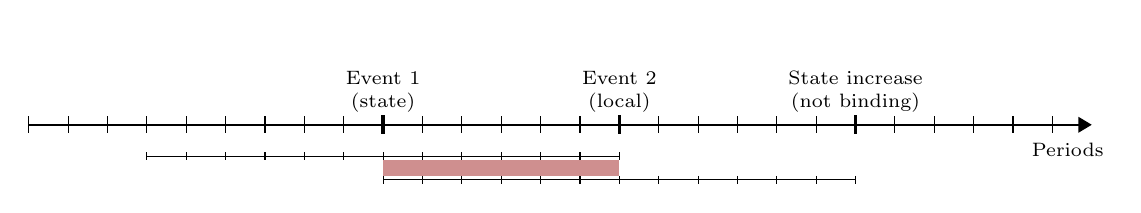
\begin{tikzpicture}
                
                %Timeline
                \draw[thick, -Triangle] (0,0) -- (13.5,0) node[font=\scriptsize,below left=3pt and -8pt]{Periods};
                    
                %Ticks and event labels
                \foreach \x in {0,0.5,...,13}
                \draw (\x cm,3pt) -- (\x cm,-3pt);
                
                \foreach \x/\descr in {4.5/\begin{tabular}{c} Event 1 \\ (state) \end{tabular}, 7.5/\begin{tabular}{c} Event 2 \\ (local) \end{tabular}, 10.5/\begin{tabular}{c} State increase \\ (not binding) \end{tabular}}
                \node[font=\scriptsize, text height=5ex, text depth=.5ex] at (\x,.7) {$\descr$};
                
                \draw[very thick] (4.5 cm,3.5pt) -- (4.5 cm,-3.5pt);
                \draw[very thick] (7.5 cm,3.5pt) -- (7.5 cm,-3.5pt);
                \draw[very thick] (10.5 cm,3.5pt) -- (10.5 cm,-3.5pt);
                
                %event windows
                \draw (1.5, -.4) -- (7.5, -.4);
                \draw (4.5, -.7) -- (10.5, -.7);
                
                \foreach \x in {1.5,2,...,7.5}
                \draw (\x cm,-.35) -- (\x cm,-.45);
                \foreach \x in {4.5,5,...,10.5}
                \draw (\x cm,-.65) -- (\x cm,-.75);
                    
                %overlap area
                \draw[lightgray!75!red, line width=5.5pt] (4.5,-.55) -- +(3,0);
                    
            \end{tikzpicture}
            \caption{Overlapping windows}
        \end{subfigure}\\
        \begin{subfigure}{1\textwidth} \centering
            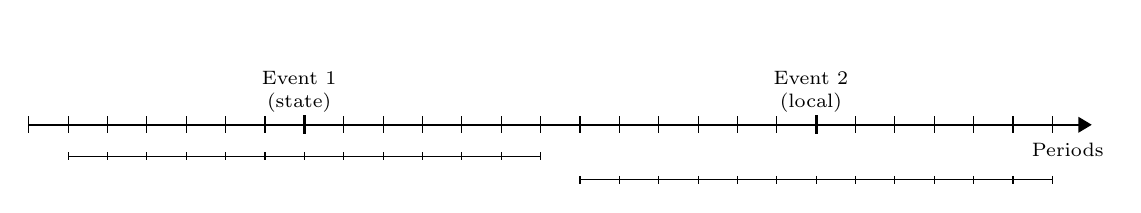
\begin{tikzpicture}
                
                %Timeline
                \draw[thick, -Triangle] (0,0) -- (13.5,0) node[font=\scriptsize,below left=3pt and -8pt]{Periods};
                    
                %Ticks and event labels
                \foreach \x in {0,0.5,...,13}
                \draw (\x cm,3pt) -- (\x cm,-3pt);
                \foreach \x/\descr in {3.5/\begin{tabular}{c} Event 1 \\ (state) \end{tabular}, 10/\begin{tabular}{c} Event 2 \\ (local) \end{tabular}}
                \node[font=\scriptsize, text height=5ex,
                    text depth=.5ex, text width=1.5cm] at (\x,.7) {$\descr$};
    
                \draw[very thick] (3.5 cm,3.5pt) -- (3.5 cm,-3.5pt);
                \draw[very thick] (10 cm,3.5pt) -- (10 cm,-3.5pt);
                
                %event windows
                \draw (.5, -.4) -- (6.5, -.4);
                \draw (7, -.7) -- (13, -.7);
                
                \foreach \x in {0.5,1,...,6.5}
                \draw (\x cm,-.35) -- (\x cm,-.45);
                \foreach \x in {7,7.5,...,13}
                \draw (\x cm,-.65) -- (\x cm,-.75);
                    
            \end{tikzpicture}
            \caption{Undefined off window dummies}
        \end{subfigure}
        \caption{An illustration of the multiple events problem in event-studies}
        \label{fig:multiple-events-example}
    \end{figure}
    
    We are currently working on two different ways to address these issues. Firstly, we are considering a model with ``infinite'' relative time dummies, in the spirit of \textcite[][, equation 1]{borusyak2017revisiting}. Secondly, we are working on a ``stacked'' event study framework, similar to \textcite{cengiz2019effect}, in which one selects as a sample a time window around each event a constructs a panel coded by event-relative time. In the first case the ``off window'' dummies do not need to be constructed, whereas in the second there are well-defined pre- and post-periods for each event. Thus, both are ways to solve the implementation problems. To control for overlapping-windows, we will add dummies for other MW changes that take place within each of the main events used for the analysis.
    
    We are working on both of the before-mentioned alternatives. As a temporary workaroudn, we deliberately selected one event per zipcode to run a traditional event-study. This brings its own complications, as discussed below. But first, let us introduce the framework that we used for the results shown in this draft.

\subsubsection{An event-study with one event per zipcode}

    One way to sort out the difficulties that arise from the multiple-events problem is simply selecting one event per unit to run a tradition two-way fixed effects specification. In this initial draft, we take this approach.  Specifically, we select the last MW increase within each unit. We do this because Zillow adds zipcodes over time, and so closer to the end of panel the more units with valid rents data we have.\footnote{We also impose the restriction that the event must have a complete window of $w$ months after it.}
    
    The estimating equation is
    \begin{equation}\label{eq:last-event-study}
        \begin{split}
            y_{jct} = & \gamma_{j} + \alpha_{ct} + \boldsymbol{\beta} \boldsymbol{X}_{jct} \\
            & + \delta^{-} D_{jct}^{-} + \sum\limits_{k = -w}^{-2}\delta_{t + k}D_{jct}^k + \sum\limits_{k = 0}^{w}\delta_{t + k} D_{jct}^k + \delta^{+} D_{jct}^{+} + \epsilon_{jct} 
        \end{split}   
    \end{equation}
    where, as before, $\gamma_{j}$ and $\alpha_{ct}$ are fixed effects; $D_{jct}^k$ is an indicator for a minimum wage taking place $k$ periods relative to $t$; and $\{D_{jct}^{-}, D_{jct}^{+}\}$ are indicators for pre- and post-event --note that we omit the indicator for the month prior to the event--. The coefficients of interest are $\{\delta_{t-w}, ..., \delta_{t-2}$, $\delta_t$, $\delta_{t+1}, ...$, $\delta_{t+w}\}$, which show the dynamics of the outcome variable around selected MW events. This equation is not free of identification problems, of course. We will discuss some of those in the next subsection.
    
    Before moving to discussing identification, two important notes about the regression equation \eqref{eq:last-event-study}. First of all, the fact that different zipcodes have a different number of accumulated MW increases means that they may also differ in the level of rents and, potentially, different dynamics. We partially account for this by including indicators for different values of the cumulative sum of unused events in the controls $\boldsymbol{X}_{jct}$.\footnote{For example, suppose a zipcode has two MW increases before the last event, at periods $\tau_1$ and $\tau_2$. In that case, we would include indicators for the period before any event $\mathds{1}\left(t \leq \tau_1\right)$, the period between the first and the second $\mathds{1}\left(\tau_1 <  t \leq \tau_2 \right)$, and an indicator after the second event $\mathds{1}\left(t > \tau_2\right)$. In here, $\mathds{1} \left( \cdot \right)$ is the indicator function.} Secondly, the set of ``last MW events'' is obviously a selected sample of all the events. For example, these events are more likely to be local. This qualifies the interpretation of the results.

\subsubsection{Identification issues}
    
    \paragraph{The ideal model}
    
    Suppose we overcome the implementation issues discussed above, and so the model in equation \eqref{eq:ideal-event-study} can be estimated. Those results will be interpretable as the ``causal'' effect of the minimum wage on rents if the following identifying assumption holds: $$E \left[ \epsilon_{jct} D_{jct}^k \big| \gamma_j, \alpha_{ct}, \boldsymbol{\beta} \boldsymbol{X}_{jct}\right]  = 0 \ \ \ \ \forall k\in\{-w, ..., 0, 1, ..., w\}. $$ This means that unobservable determinants of the outcome are mean independent from the relative timing of the MW event conditional on the set of fixed effects and controls. We can also interpret this assumption as ``parallel-trends'', meaning that, in the absence of some minimum wage change, the counterfactual outcome between units treated at different times within a given county would have not differed systematically.
    
    Given that equation \eqref{eq:ideal-event-study} utilizes within zipcode variation to pin-down the effect, this assumption seems much more plausible than the assumptions needed when using within county variation and a much less flexible set of fixed effects. Conditional on county-specific time fixed effects and county-specific calendar months,\footnote{Note that these fixed effects are a very high dimensional object.} the unobserved within zipcode variation is unlikely to be correlated with the determinants of the timing of the MW change, as these are not likely to be determined at the zipcode level. One important reason for this is that MW changes are usually enacted through federal or state law, or through local ordinances that are subject to higher level court blocks and revisions, and that may follow from ballot initiative. Therefore, the timing of the enactment of a MW change in a given zipcode could be thought as random. Furthermore, we control for flexible local business cycles, alleviating concerns about differential trends when introducing a minimum wage.\footnote{Suppose political units, such as states and counties, introduce a minimum wage at the same time when they are experiencing an economic boom. Estimation of this model will exploit variation within county, after controlling for the business cycle. These kind of concerns are thus misplaced in this context.}
    
    \paragraph{The last event specification}
    
    Restricting the pool of events used for estimating the treatment effect to one per unit, however, introduces different identification issues as pointed out by \textcite{borusyak2017revisiting}. Specifically, the identification of a dynamic causal effect is hampered by the impossibility of separately estimate relative time and period fixed effects, as each of them occur only once per unit, making it impossible to pin it down up to a linear trend. One possible solution is to remove the unit fixed effects at the expenses of a stronger identification assumption and less power. We perform this by running an alternative specification of \eqref{eq:last-event-study} where we replace zipcode-level fixed effects with county-level ones. Under this new framework, the identifying assumption becomes $E \left( \epsilon_{jt} D_{j(t+k)} | \alpha_c, \alpha_{ct}, \boldsymbol{\beta} \boldsymbol{X}_{jt}\right)  = 0  \ \ \ \forall k\in[-w, w]$. Altought we include a third-degree polynomial for time trend as additional controls, note that we are still allowing for the possibility of having unobserved time varying trends correlated both with MW changes and with prices. 
    
    In addition to this, we then introduce a further specification with a control group made of zipcode that do not experience changes in MW in our sample [ADD EQUATION FOR CLARITY?]. This allows us to separately pin down year effects from the causal treatment effect of MW changes by the very fact that such units are indeed never treated. Note that, in order to test the strength of our results, we can add county-level trends since such geographical unit does not perfectly overlap with treated and control group. \\   

\subsection{First-difference specifications}\label{subsec:empirical_strategy/first-difference}

\subsubsection{Static model}

    Following \textcite{meer2016effects} : 
    
    \begin{equation}\label{eq:diff_main}
        \Delta \tilde{y}_{jt} = \sum\limits_{k = -5}^{5} \delta_{t+k} \Delta \tilde{D}_{j(t+k)} + \alpha_{t} + \boldsymbol{\beta} \boldsymbol{X}_{jt} + \nu_{jt}
    \end{equation}
    
    where $\Delta \tilde{y}_{jt}$ and $\Delta \tilde{D}_{j(t+k)}$ are the first difference of log outcome and MW respectively. Note that the first difference specification already take care of the unit fixed effect, hence not included. Identification in the current setting is reached assuming changes in the outcome variable that are invariant up to a linear transformation \parencite{borusyak2017revisiting}. In [RESULTS] we show how the county-level FE version of \autoref{eq:main_ziplevel} indeed reveals a sudden jump in the outcome vairable at treatment time along with a fairly linear dynamic hence justifying the validity of this latter approach. 
    
    We will discuss the no pre-trends assumption in the next section.


\subsubsection{Dynamic model}

    Lala
    

\subsection{Towards the effect of wages on rents}

    An object that is also of interest is the effect of wages in a local neighborhood on the rents paid by individuals living there, going beyond the minimum wage. In the future, we would like to estimate this parameter via a TSLS system, where we instrument wages with the minimum wage.


\section{Preliminary Results}\label{sec:results}

\subsection{Rents}

Figure \ref{fig:fig1}\footnote{Code producing the analysis in this section can be found in \url{https://github.com/diegogentilepassaro/min_wage_rent}} plots the relative event coefficients of a regression like (1) for single family rents per square foot for MW events of at least \$0.5. 

\begin{figure}[h!]
    \centering
    \scalebox{0.45}{
    \includegraphics{draft_june20/figures/medrentpricepsqft_sfcc_last_sal_mw_event_rel_months6}
    }
    \caption{Baseline specification. Effects of a MW change of at least \$0.5 on single family rent per square foot (in dollars). Standard errors are clustered at the zipcode level.}
    \label{fig:fig1}
\end{figure}

The average increase of the MW change in this specification is of \$0.8. For a family of 2 minimum wagers that work 40 hours a week, given that the average month has 4.35 weeks, this change represents an increase on the family income of \$278.4. The on-impact effect on rents per square foot is of around ten cents and grows slightly in the months following the event. Assuming this representative single family consumes 1500 square feet of housing, the implied increase in monthly rent is of about \$150, which implies an on-impact pass-through from the MW change to rents of 53.9\%. If assuming that the treatment effect is given by averaging the 7 post event coefficient, then the implies pass-through is of about 64.4\%.

First note that, taken at face value this number seems slightly high given that the  median US rent requires 28.4\% of the median incomes \parencite{bi}. However, a household with 2 full time minimum wagers making, for example, the federal minimum wage of \$7.25 will have an annual income of \$30276, only slightly above half of the median US household income of \$59430 in 2015, which suggests that the estimated pass-through is plausible. 

Second, we check the robustness of this result by change the prominence of the MW changes. We use MW changes that comply to our sample criterion (explained in section 2) and are of at least \$0.25 and of at least \$0.75 instead of \$0.5. For each of the event definitions we bootstrap, clustering at the zipcode level, the whole computation of the pass-through (assuming that the relevant per square foot effect is the average of the post event coefficients). The results are presented in Table \ref{tab:table1}, where the middle column corresponds to Figure \ref{fig:fig1}. Note that we compute the implied pass-through for 3 different housing size assumptions: 1000, 1500, and 2000 square feet. We believe that those 3 values cover the range of plausible values for the average rental of a single family with 2 MW earners. Finally, note that as in any event-study, we are using only the zipcodes that have at least one MW change in our period. To gain precision, and for further robustness we are planning to use a specification that allows us to also use zipcodes that never have a MW change. Intuitively, this will help us estimate the fixed effects more precisely. 

\begin{table}[h!]
    \centering
    \resizebox{\textwidth}{!}{
    {
\def\sym#1{\ifmmode^{#1}\else\(^{#1}\)\fi}
\begin{tabular}{l*{3}{c}}
\hline\hline
            &\multicolumn{1}{c}{(1)}        &\multicolumn{1}{c}{(2)}        &\multicolumn{1}{c}{(3)}        \\
            &\multicolumn{1}{c}{MW changes of at least \$0.25}&\multicolumn{1}{c}{MW changes of at least \$0.5}&\multicolumn{1}{c}{MW changes of at least \$0.75}\\
\hline
Rent increase per square feet&                0.0216\sym{*}  &                 0.103\sym{***}&                0.0812\sym{***}\\
            &      [0.00126,0.0420]         &        [0.0434,0.162]         &        [0.0540,0.108]         \\
[1em]
Total rent increase (assuming 1000 square feet)&                 21.62\sym{*}  &                 102.6\sym{***}&                 81.19\sym{***}\\
            &         [1.264,41.97]         &         [43.40,161.8]         &         [53.96,108.4]         \\
[1em]
Total rent increase (assuming 1500 square feet)&                 32.43\sym{*}  &                 153.9\sym{***}&                 121.8\sym{***}\\
            &         [1.896,62.96]         &         [65.10,242.7]         &         [80.93,162.6]         \\
[1em]
Total rent increase (assuming 2000 square feet)&                 43.24\sym{*}  &                 205.2\sym{***}&                 162.4\sym{***}\\
            &         [2.528,83.94]         &         [86.80,323.7]         &         [107.9,216.9]         \\
[1em]
Increase in income of a household with 2 full time minimum wages&                 219.2\sym{***}&                 278.4\sym{***}&                 403.7\sym{***}\\
            &         [211.5,227.0]         &         [269.1,287.7]         &         [388.0,419.3]         \\
[1em]
Implied passthrough from MW to rents (assuming 1000 square feet)&                0.0986\sym{*}  &                 0.369\sym{***}&                 0.201\sym{***}\\
            &       [0.00523,0.192]         &         [0.156,0.581]         &         [0.133,0.269]         \\
[1em]
Implied passthrough from MW to rents (assuming 1500 square feet)&                 0.148\sym{*}  &                 0.553\sym{***}&                 0.302\sym{***}\\
            &       [0.00784,0.288]         &         [0.235,0.871]         &         [0.199,0.404]         \\
[1em]
Implied passthrough from MW to rents (assuming 2000 square feet)&                 0.197\sym{*}  &                 0.737\sym{***}&                 0.402\sym{***}\\
            &        [0.0105,0.384]         &         [0.313,1.161]         &         [0.266,0.539]         \\
\hline
Average MW change&                   .63         &                    .8         &                  1.16         \\
Number of zipcode-months&                 68713         &                 43716         &                 37837         \\
Number of Zipcodes&                   676         &                   440         &                   383         \\
Number of bootstrap repetitions&                   196         &                   199         &                   196         \\
\hline\hline
\end{tabular}
}

    }
     \vspace{1ex}
    {\raggedright Square brackets display the 95\% bootstrapped confidence intervals. Income computations are done assuming 2 MW earners.\par}
    \caption{Bootstrapping the main objects of interest}
    \label{tab:table1}
\end{table}

Next, we show the importance of allowing for flexible year-month fixed effects that are specific to the county. Remember that is was not feasible when the unit of observation is the county. If we just include two-way fixed effects, which in our case corresponds to zipcode and year-month, all variation across time and zipcodes will end up being used estimating the relative event coefficients. But if, for example, different states or counties or MSAs have different time trends in rent prices, as it is probably the case, then the model will be misspecified. In particular, as within zipcode variation is not "de-trended", the relative event coefficients will be much harder to estimate as they will be cofounded by the trend. Figure \ref{fig:fig2} presents an event study plot analogous to Figure \ref{fig:fig1} but using a simple two-way fixed effect specification. 

\begin{figure}[h!]
    \centering
    \scalebox{0.45}{
    \includegraphics{draft_june20/figures/two_way_rent_sfcc.png}
    }
    \caption{Two-way fixed effects specification. Effects of a MW change of at least \$0.5 on single family rent per square foot (in dollars). Standard errors are clustered at the zipcode level.}
    \label{fig:fig2}
\end{figure}

In fact, we see that estimation of the relative coefficients is much noisier and lower in magnitude. The within variation R-squared (the percentage of the within variation in the data explained by the model) is of 0.0066. When allowing for county-specific time fixed effects and county-specific calendar months (to allow for flexible seasonality patterns) that are infeasible under the specifications in the previous literature we get \ref{fig:fig1} and a within variation R-squared of 0.0779, so that we are able to explain 12 times more within zipcode variation. These results suggest that county-specific year-month and seasonal month variation are important determinants of monthly rent at the local level above and beyond two way fixed effects.

The last result of this subsection shows what happens if we aggregate our zipcode-month data at the county-quarter level\footnote{In order to use the data in the same unit as \textcite{tidemann2018mw,yamagishi2019minimum} we should have aggregated at the county-year. However, that involves dealing with overlap in the events for each county as we have many MW changes on subsequent years. Therefore, we aggregated the data at the county-quarter under the thought that we can only do better than at the county-year. }. Figure \ref{fig:fig3} plots the relative event coefficients for a two-way fixed effect specification at the county-quarter, for a window of 2 quarters around MW changes of at least \$0.5. Similar to \textcite{tidemann2018mw} results are very imprecise and point estimates are, if anything, negative. 

\begin{figure}[h!]
    \centering
    \scalebox{0.45}{
    \includegraphics{draft_june20/figures/medrentpricepsqft_sfcc_last_sal_mw_event_rel_quarters2.png}
    }
    \caption{Two-way fixed effects county-quarter specification. Effects of a MW change of at least \$0.5 on single family rent per square foot (in dollars). Standard errors are clustered at the zipcode level.}
    \label{fig:fig3}
\end{figure}

\subsection{House Prices}

Figure \ref{fig:fig1} plots the relative event coefficients of a regression like (1) for single family house values per square foot for MW events of at least \$0.5. 

\begin{figure}[h!]
    \centering
    \scalebox{0.45}{
    \includegraphics{draft_june20/figures/medlistingpricepsqft_sfcc_last_sal_mw_event_rel_months6.png}
    }
    \caption{Baseline specification. Effects of a MW change of at least \$0.5 on single family house prices per square foot (in dollars). Standard errors are clustered at the zipcode level.}
    \label{fig:fig4}
\end{figure}

The effect on house values per square foot is of around \$12.5. If we take a purely financial perspective that house values are the present discounted value of perpetuity, we can compute the implied interest rate from the increase in the per square foot present discounted value of \$12.5 (heareafter PDV) and the increase in a monthly cash flows of around \$0.10 cents from section 4.1 (hereafter CF).

\begin{equation}
    PDV = \frac{CF}{r} \to r = \frac{CF}{PDV}
\end{equation}

For our case, the implied monthly interest rate is of 0.008 which implies an annual interest rate of around 10\%. This seems like a very high interest rate, although is not totally implausible. It could potentially be rationalized if agents also expect capital gains on the house, or if agents are also capitalizing future MW changes (as they might expect that a MW change in a given location means that more MW changes may come in the future). Further analyzing these results is work for the future. 

\subsection{Amenities}

For the future. 


\section{Conclusions}

For the future.

\nocite{*}
\printbibliography


% \begin{figure}[h!]
% \centering
% \begin{subfigure}{.5\textwidth}
%   \centering
%   \includegraphics[width=.8\linewidth]{rent2br_median_rel_months_min_event12.png}
%   \caption{12 month window}
%   \label{fig:sub1}
% \end{subfigure}%
% \begin{subfigure}{.5\textwidth}
%   \centering
%   \includegraphics[width=.8\linewidth]{rent2br_median_rel_months_min_event24.png}
%   \caption{24 month window}
%   \label{fig:sub2}
% \end{subfigure}
% \caption{Median rent for a 2 bedroom}
% \label{fig:test}
% \end{figure}

% \begin{figure}[h!]
% \centering
% \begin{subfigure}{.5\textwidth}
%   \centering
%   \includegraphics[width=.8\linewidth]{rent2br_psqft_median_rel_months_min_event12.png}
%   \caption{12 month window}
%   \label{fig:sub1}
% \end{subfigure}%
% \begin{subfigure}{.5\textwidth}
%   \centering
%   \includegraphics[width=.8\linewidth]{rent2br_psqft_median_rel_months_min_event24.png}
%   \caption{24 month window}
%   \label{fig:sub2}
% \end{subfigure}
% \caption{Median rent per square foot for a 2 bedroom}
% \label{fig:test}
% \end{figure}

\end{document}